\chapter{Overview of Hardware \& Technologies}

Due to the explorative nature and the width of this thesis, we have to introduce a variety of different IoT ISA's, System-on-a-Chip manufactureres and their relevant products, open source projects with the aim to aid in the process of embedding, toolchains, and technologies. This chapter serves as an overview of the various devices and tools that were discovered, and may help further research which aim to achieve similar goals.

\section{Micro Computing}
Von Neumann's Architecture states that a modern computer requires a couple of core components to be able to run~\cite{arikpo2007neumann}. Figure \ref{fig:vonNeumanng} shows a visual representation.
\begin{itemize}
\item A \textbf{Processor Unit}, or a \textbf{core processing unit (CPU)} can further be divided into two subcomponents, the Controll Unit (CU) and the Arithmetic Logic Unit (ALU). This component performs operations and instructions on the data stored in the main memory unit and on the I/O devices.
\item The \textbf{Main Memory Unit}, or simply memory, stores data and the operations that need to be performed on this data.
\item The \textbf{Input/Output (I/O) Devices}, can be anything that allows us to interact with the computer, such as a mouse or keyboard, or simply just an LED light that gets turned on.
\end{itemize}

\begin{figure}
\centering
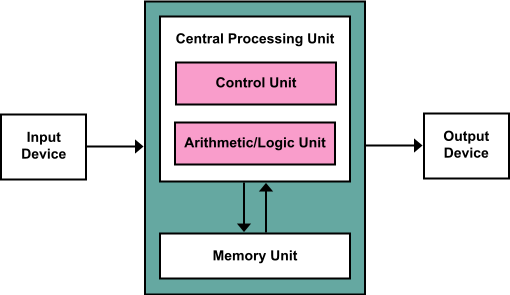
\includegraphics[width=0.6\textwidth]{Von_Neumann_Architecture.png}
\caption{Von Neumann Architecture~\cite{vonNeumanngfx}}
\label{fig:vonNeumanng}
\end{figure}

We can apply the definition of Von Neumann's Architecutre to further categorize two IoT edge devices:
\begin{itemize}
\item A \textbf{Micro controller unit (MCU)} is an integrated, fully capable, self sufficient computer on a sincle chip. It can run a "bare metal interface", meaning that it doesn't require to run an OS. Without which, it can run a single thread, or a controll loop, forever. As the title of this thesis implies, MCUs are the main focus of this thesis. 
\item A \textbf{Micro processor unit (MPU)} requires support from surrounding chips that enable various functionalities like memory, interfaces, and I/O and cannot act as a stand alone computer. The MPU, according to the Von Neumann's Architecture, is just the processor unit.
\end{itemize}
While the above terms, MCU and MPU, are oftentimes used interchangably, we want to point out the differences of these two families. It is far easier to run an OS such as the Linux Kernel \cite{raspberrypios} on MPU enabled devices, such as the Raspberry Pi 4, because it is not limited to the capabilites on the chip, and can easily be extended with, i.e. more RAM~\cite{raspberrypi4}. A MCU is limited to the design and capabilities of the chip. Hence, a MPU runs with far higher processing capability and much larger applications, while MCUs are for lightweight computing where the OS, if one decides to use one, is integrated on-chip. 
But because some MCUs have straightforward software drivers for more complex peripherals and more MPUs are available that have integrated peripherals on-chip, the gap between MCUs and MPUs is becoming less evident~\cite{peterson2021mcu, thornton2017mcu}.
%

\section {Processors}
When compiling software for a target platform, one must be aware of the different instruction set architectures (ISA) of the target CPUs. Listed below are the most noteworthy processor families that we came across.

\begin{itemize}
\item \textbf{ARM Cortex-M-Series}, are 32-bit RISC processors, designed for low-cost, low-power, and usually embedded in MCUs and other IoT devices~\cite{cortexm}.
\item \textbf{ARM Cortex-A-Series}, are 32-bit or 64-bit RISC processors, in contrast to the Cortex-M-Series, these processors have higher energy consumption that are built for more complex tasks such as supporting an OS~\cite{cortexa}.
\item \textbf{Tensilica Xtensa}
\end{itemize}

As description of the ARM Cortex-M processors seems to fit our premise perfectly, the low-cost and MCU aspect, we will focus on these types of CPUs


\section{Market Analysis}

[MAYBE MOVE THIS CHAMPTER TO THE IMPLEMENTATION?]

To find a suitable MCU that could support Linux, a market analysis had to be performed. The most relevant criteria where having sizable RAM preferably more than 1MB, more than 40MHz CPU clock rate, availability in the region, and a large community because this can simplify development due to the availability of online ressources. Furthermore with the homogenious nature of IoT, directing this thesis towards a smaller target audience would inevitably decrease its value.

\begin{sidewaystable}[]
	\centering
	\begin{tabular}{c|c|c|c|c|c|c|c|c}

	\textbf{Manufacturer} 	& \textbf{Chip/Dev Board} & \textbf{Classification} & \textbf{CPU} & \textbf{ISA} & \textbf{bit} & \textbf{Clock rate} & \textbf{RAM} & \textbf{Flash} \\
	\hline
	\hline
	Raspberry Pi          	& Raspberry Pi 4   	& MPU  	& ARM          & Cortex-A72   	& 64    	& 1.5GHz		& 2-8GB (SDRAM)		& asdf\\
	Raspberry Pi          	& Zero 2 W          	& MPU   	& ARM          & Cortex-A53   	& 64     	& 1GHz		& 512MB (SDRAM)		& asdf\\
	Raspberry Pi          	& Pico           		& MCU   	& ARM          & Cortex-M0+   	& 32 	& 133 MHz 	& 264kB (SRAM)	 	& 2MB\\
	\hline
	Espressif             		& ESP32               & MCU   	& Tensilica    	& Xtensa       		& 32		& 240 MHz	& 520kB (SRAM)		& adsf\\
	Espressif             		& ESP32-S2    	& MCU   	& Tensilica    	& Xtensa       		& 32		& 240 MHz	& 320kB (SRAM)		& asdf\\
	Espressif             		& ESP32-C3    	& MCU   	& RISC-V       & RISC-V       	& 32		& 160 MHz	& 400kB (SRAM)		& asdf\\
	Espressif             		& ESP32-S3     	& MCU   	& Tensilica    	& Xtensa       		& 32		& 240 MHz	& 512kB (SRAM)		& asdf\\
	\hline
	STMicroelectronics  	& STM32F0     	& MCU   	& ARM          & Cortex-M0    	& 32		& 48MHz		& 4-32kB				& asdf\\
	STMicroelectronics  	& STM32F1     	& MCU 	& ARM          & Cortex-M3    	& 32		& 72MHz		& 4-94kB				& adsf\\
	STMicroelectronics  	& STM32F3       	& MCU  	& ARM          & Cortex-M4    	& 32		& 72MHz		& 16-80kB (SRAM)		& asdf\\
	STMicroelectronics  	& STM32F4       	& MCU  	& ARM          & Cortex-M4    	& 32		& 180MHz	& 256kB (SRAM)		& asdf\\ % correct this
	STMicroelectronics  	& STM32G0        	& MCU  	& ARM          & Cortex-M0+   	& 32		& 64MHz		& 144KB (SRAM)		& asdf\\
	STMicroelectronics  	& STM32L4       	& MCU   	& ARM          & Cortex-M4    	& 32		& adsf		& adf 				& adf\\ % correct this
	STMicroelectronics  	& STM32G4       	& MCU   	& ARM          & Cortex-M4    	& 32		& 170 MHz	& 128-512KB (CCM-SRAM)& asdf\\ % correct this
	\hline
	Arduino               		& Due A000062    	& MCU  	& ARM          & Cortex-M3    	& 32       & 84MHz		& 96KB (SRAM)		& asdf \\         
	\end{tabular}
	\caption{Market analysis of available IoT edge devices}
	\label{tab:market}
\end{sidewaystable}

With the insights of the market analysis, see table \ref{tab:market}, and the realization that the required MCU on-chip RAM might not suffice for running Linux, a multitude of sales representatives of hardware manufactureres primarily of STM, were contacted. Among others, Digi-Key Electronics, Anatec AG, Avnet Silica Rothrist and Mouser Electronics. Questions concerning extensibility of RAM were posed with the goal of gaining expert insight. For the purposes of this thesis, more RAM was required.

[MENTIONE: I arranged the boards from STM to get some support.]

\begin{figure}
\centering
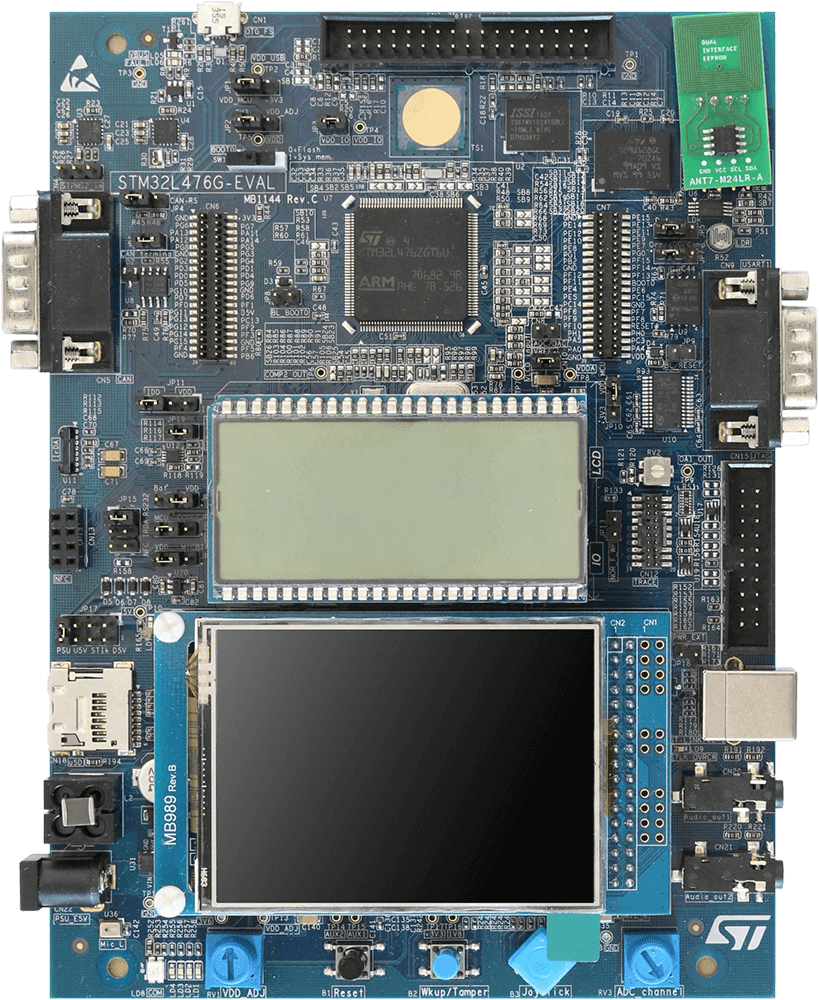
\includegraphics[width=0.6\textwidth]{stm32l476g-eval.png}
\caption{STM32L476G-Eval development board~\cite{stm32Lpic}}
\label{fig:stm32l}
\end{figure}
THE PICTURE ------>\cite{stm32Lpic} \figref{stm32l}

[ADD PICTURE OF THE ESP32 WROOWIE]

\section{Toolchains, Cross-Compilation \& Libraries}\label{toolchains}
For compiled languages, the appropriately name toolchain combines multiple steps into a single pipeline, to produce binary, or machine code. Each step in the process is a piece of software that fullfils its role or function, and hands work over to the next tool in the chain. Interpreted languages such as Python do not require compilation or toolchains, the interpreter executes, or interprets, the code directly. Since this thesis focuses on code than runs closely to hardware, interpreted languages are not concidered. When compiling code a multitude of factors need to be concidered when choosing a toolchain, because they are specifically designed to work excusivley in the right circumstances. Most importantly, whether the host platform is the same as the target platform. The host is the platfrom on which the compilation takes place, and the target on which the binaries will evenually end up running on. If host and target platfrom are not the same, then we speak of cross-compilation. Another important aspect of cross-compilation is the fact that, especially in our case, the target platform may lack computing power and memory, thus compiling could be very time inefficient or simply be impossible. If compilation in mentioned, cross-compilation is implied, since the goal of this thesis is not to evaluate binary code compiled for the host system, but for the target system, being the MCU edge devices. Broadly simplified toolchains work as follows.

As mentioned, the first tep in a toolchain is source code compilation. Depending on the programming language the source code was writen in, compiler vary. For different compiled languages such as C and C++ different compilers are required. In our case, C is of primary concern because the linux kernel is mostly (98.4\%) written in C~\cite{githubLinux}. From each source file that was compiled in the first step result Assembly code. Assembly code, marked with ending \code{.s}, is a set of simplified instructions and basic operations, in other words its a human readable abstraction of maschine code, i.e. bits.
Nowdays Assembler programming is only utilized in situations when extremely efficient management of processor activities is required, but it is still an intermediate-product in compilation. Assebly code needs to be assembled outputing object code. Finaly the object code files need to be linked with required libraries to form an, either statically or dynamically linked, executable, see section \ref{dsll}. After successful cross-compilation follows only execution on target device, which might seem like the easiest step, this is further discussed in section \ref{flashing.ch}.

For the goals of this tesis, we will be compiling, mostly, C code on host platform operating on \code{x64} architecture for target platforms on \code{Armv7E-M} architecutre. Hence cross-compilation will take place with the \code{gcc-arm-none-eabi} toolchain~\cite{gcc-arm-none-eabi}.

[INCLUDE GRAPHIC FOR COMPILATION]

\subsection{Dynamically \& Statically Linked Libraries}\label{dsll}
A Library is a collection of precompiled and reusable components that hold functionality for common processes. The most common example for such a library is C's \code{stdio.h} which hold, among others, function \code{fprintf}, which simply prints characters to the console. As previously stated there are two main methods of linking such functions with the executables, we distinguish between statically linked libraries (SLL) or static libraries, and dynamically linked libraries (DLL) or shared libraries. SLL is the simplest form, as when linking, the contents of the library, specifically the required functions, are included in the executable file. On a small scale this doesn't pose any problems, yet with more exectuables that are loaded into memory, each of these executables contain their own SLL. This can lead to the RAM (or ROM) being occupied by the same function multiple times. Especially when RAM is limited, as is in our case, the redundancy of the same function is not desired. DLL on the other hand requires only one instance of the functionality, all the executables that require this specific function, can access the read-only segment of the library, therefore it can be shared. This process of sharing libraries is aided by a hardware solution, the MMU, see section~\ref{mmu.ch}.

Once again, for our purposes dynamically linked executables are required, since we want to save as much space as possible, thus only linking the required functions and not the entire library. 
%

\subsection{Buildroot }\label{buildroot.ch}
Buildroot is a tool that makes cross-compiling a complete Linux system for an embedded devices easier and more automated. It runs primarily on Linux systems. Through the use of this facilitated toolchain, it creates a self compressing version of the Linux kernel \code{zImage}, a root filesystem, a U-boot bootloader, and root file system and an SD card image file \code{sdcard.img}~\cite {buildroot}.

\subsection{Yocto Project \& OpenWrt}
Equivalently to Buildroot, the Yocto Project and OpenWrt are tools used for Linux cross-compilation for embedded systems. OpenWrt has a focus on Netoworking, the Yocto Project does not currently support MMU-less builds.~\cite{openwrt, yocto}. These tools are not used in this thesis but fill a similar role as Buildroot and are mentioned for the sake of thoroughness. 

\section{Memory Management Unit}\label{mmu.ch}
The Memory Management Unit (MMU) is hardware that is positioned between the processor and physical memory. If present, memory references from the software, through the processor, are passed through the MMU, which in turn maps these references to the actual memory, where the data being called actually resides. In more techtical terms, the reference points to a virtual memory addresses that the MMU can translated into the physical memory addresses. Hence, the program running on the CPU can doesn't need to know the physical memory address. This can simplify addressing in complicated systems. Furthermore, the MMU facilitates DLL implementation. Linux's memory management system is very complicated and has grown over time, offering a growing number of features, such as \code{nommu} which means MMU-less devices, often MCUs~\cite{linuxMMU1, linuxMMU2}. While the implementation of DLL, for devices that don't contain a MMU device appears to be possible, it once again is very complicated~\cite{sharedLibnoMMU}. There exits Linux variations that are tailored for MMU-less devices, see section~\ref{uclinux}

\section{The Linux Kernel}
The Linux Kernel (Linux) was initially created, by Linus Torwalds, in 1991 for i368 based PCs. After its initial appearance it quickly gained traction among developers, and was licenced under GNU General Public License (GPL) as free OSS~\cite{linuxlicense}. At current time, Linux supports all kinds of different target architectures, and dominates that IoT market~\cite{sabri2017comparison}.


\subsection{$\mu$Clinux}\label{uclinux}
The open source nature of Linux made it possible to fork the source code and modify it according to ones needs. One such project is the $\mu$Clinux, which was specifically created to target MMU-les microcontrollers. Its hardware dependent, such as physical memory, and independent code, such as virtual memory, are distinct. Using the given instructions, the hardware-specific portion may be altered for a number of CPUs, hence the OS is modifiable. The system supports both user-space and kernel-space, and switching between the two may be done using system calls. It is possible to develop in a multi-threading environment using POSIX thread libraries. Neither a virtual memory model nor an memory protection unit exist, but functions can be used to dynamically allocate memory, hence DLL is possible. It features a complete TCP/IP stack that may be swapped out for a lighter stack like uIP or lwIP~\cite{dunkels2003full}. But, in comparison to other IoT edge device OSs, as seen in section \ref{iotos}, $\mu$Clinux has a far larger footprint than other IoT OSes~\cite{gaur2015operating}. $\mu$Clinux was eventually discontinued as a standalone fork and was reintroduced into the mainline Linux kernel. With the official emailing list gone quiet and its webpage only visible through web archives, and the last official update publish in May of 2016~\cite{uclinux.org}. Other entities appear to have forked and maintained it further down the line, such as emcraft~\cite{emcraft, emuClinux}, with last comits on December 2017, one year later. The last remaining verifiable remnants appear to be pointing towards a "small C library for developing embedded Linux systems" called uclibc-ng~\cite{uclibc-ng}, which could prove useful.

\section{U-Boot}
"Das U-Boot" is an open source boot loader used predominantly in embedded devices. It's main focus is to load the OS kernel into main memory. It supports a wide variety of IoT development boards~\cite{u-boot-doc}. Yet again, as is common in the IoT ecosystem, there is a multitude of U-Boot forks, the original and the one that appears to be maintained and updated most frequently is by denx, while the previously mentioned emcraft has their own~\cite{emUboot}. 

When not otherwise mentioned, when U-Boot is mentioned we are refering to U-Boot maintained by denx~\cite{u-boot}.

\section {QEMU}\label{qemu.ch}
Primarily a general-purpose machine virtualizer and emulator, QEMU has a variety of applications. In this thesis we will use it to emulate a system, thus creating a virtual replica of a MCU, including the CPU, memory, and simulated peripherals, in order to run a compiled version of Linux. The CPU may operate in this mode entirely emulated or in conjunction with a hypervisor like KVM, Xen, Hax, or Hypervisor. Equivalently to the cross-compilation process that was dicussed in section \ref{toolchains}, the "user mode emulation," allows QEMU to run programs that were built for the target CPU, on our host CPU~\cite{qemu}.

